\documentclass{beamer}

\mode<presentation>
{
  \usetheme{Madrid}      % or try Darmstadt, Madrid, Warsaw, ...
  \usecolortheme{rose} % or try albatross, beaver, crane, ...
  \usefonttheme{structurebold}  % or try serif, structurebold, ...
  \setbeamertemplate{navigation symbols}{}
  \setbeamertemplate{caption}[numbered]
}

\usepackage[english]{babel}
\usepackage[utf8x]{inputenc}
\usepackage{color}
\usepackage{natbib}
\usepackage{algorithm}
\usepackage[noend]{algpseudocode}
\usepackage{tikz}
\usepackage{pgfplots}
\usepackage{subfig}
\pgfplotsset{compat=1.18} % or newest available


\newcommand{\N}{\mathbb{N}}
\newcommand{\Z}{\mathbb{Z}}
\newcommand{\Q}{\mathbb{Q}}
\newcommand{\R}{\mathbb{R}}
\newcommand{\C}{\mathbb{C}}
\newcommand{\PP}{\mathbb{P}}
\newcommand{\EE}{\mathbb{E}}

\newcommand{\inv}{^{-1}}
\newcommand{\sm}{\setminus}
\newcommand{\ol}{\overline}
\newcommand{\what}{\hat w}
\newcommand{\wopt}{w_*}
\DeclareMathOperator{\Tr}{Tr} 


\title[Robust Optimization for ALR]{
    Robust Optimization in Active Linear Regression
}
\author{Khai Dong, Kyle Eng, Dylan Le}
\institute{RPI}
\date{\today}

\bibliographystyle{plainnat}

\begin{document}

\begin{frame}
  \titlepage
\end{frame}

% % Uncomment these lines for an automatically generated outline.
% \begin{frame}{Outline}
%  \tableofcontents
% \end{frame}
% \section{Background}

\begin{frame}{Motivation}
    \begin{block}{Training Cost in Examples}
    For a fixed compute budget, training a good transformer could require \(\approx\)20 tokens per parameter, so for 70B parameters we could need 1.4T tokens  
    \citep{chinchilla}. 
        
    \end{block}
    \vfill\pause
    \begin{block}{Cost of Labelling}<1->
    The average hourly rate is \$25.23 and experts can be even be paid up-to \$54.09 (40-100k annual)\citep{ziprecruiter_data_annotation_salary}.
    \end{block}
    \textbf{Can we reduce this human cost, through reducing the label complexity?}
\end{frame}
\begin{frame}{Linear Regression and Active Learning}

    \begin{block}{$\ell_2$ Linear Regression}<1->
        Given $X \in \R^{N \times d}$ and $y \in \R^{N}$. Compute $\wopt = \arg \min_{w \in \R^d} \|Xw - y \|_2^2$.
    \end{block}
    \vfill
    \begin{block}{Active Learning}<2->
        Suppose we are only given $X$, and entries of $y$ can be queried with \textbf{a cost}.
        \begin{itemize}
            \item Obtaining labels is \textbf{expensive} and slow, as they require experts (e.g., radiologists, pathologists, clinicians)
        \end{itemize}
        \vfill

    \textbf{Can we reveal less of $y$ while obtaining $\what \approx \wopt$?}
        
    \end{block}

\end{frame}

\begin{frame}{What does it means for $\what \approx \wopt$?}
    \begin{block}{Claim}<1->
        The active learning problem cannot be solved \textbf{deterministically}.
    \end{block}
    
    \only<2->{
    \begin{equation*}
        X = \begin{bmatrix}
            \textcolor{red}{1} & \textcolor{red}{0}\\
            \textcolor{red}{0} & \textcolor{red}{1}\\
            1 & 0\\
            0 & 1\\
            1 & 0\\
            0 & 1
        \end{bmatrix}
        \qquad
        y = \begin{bmatrix}
            \textcolor{red}{1}\\
            \textcolor{red}{1}\\
            0\\
            0\\
            0\\
            0
        \end{bmatrix}
    \end{equation*}
    }
    \begin{block}{Claim}<3->
        If the algorithm deterministically removes the red rows, we lose all information.
    \end{block}
\end{frame}

\begin{frame}{What does it means for $\what \approx \wopt$?}

    \begin{block}{$\epsilon$-regret}<1->
        Suppose $\what$ is drawn from some distribution $\mu$.\\ 
        $\what$ approximates $\wopt$ with $\epsilon$-regret if
        $
            \EE_{\mu}[\lVert X\what - y \rVert_2^2] \leq 
            (1+\epsilon) \cdot \lVert Xw_* - y \rVert_2^2.
        $
    \end{block}

    \begin{block}{Coreset}<2->
        For most known methods, we sample a coreset, i.e., a subset of (rescaled) rows $(A, y_A)$  of $(X, y)$, and take $\what = \arg \min_{w} \| Aw - y_A \|_2^2$.
    \end{block}


    % \begin{block}{Main Focus}<3->
    %     We will focus on $\epsilon = d/N$ to preserve the benefits of using \textbf{all} of $X$ while using \textbf{less} of $y$~\citep{Mostafa2012}.
    % \end{block}
    
\end{frame}

\begin{frame}{Coreset}

\centering
\begin{tikzpicture}
\begin{axis}[
    width=0.85\textwidth,
    height=0.65\textwidth,
    xmin=0, xmax=10,
    ymin=0, ymax=12,
    xlabel={$x$},
    ylabel={$y$},
    grid=both,
    legend pos=north west,
]

% -------------------------
% Full dataset (noisy)
% -------------------------
\addplot[
    only marks,
    mark=*,
    blue,
    opacity=0.3,
    mark size=2.5pt,
]
coordinates {
    (1,0.6) (2,2.4) (3,2.0) (4,4.7) (5,4.1)
    (6,6.6) (7,5.8) (8,9.2) (9,8.0)
};


% -------------------------
% Coreset (random sample)
% -------------------------
\addplot[
    only marks,
    mark=*,
    red,
    mark size=3.5pt,
]
coordinates {
    (2,2.4) (5,4.1) (8,9.2)
};


% -------------------------
% Full-data regression line
% -------------------------
\addplot[
    domain=0:10,
    dashed,
    thick,
    blue,
]
{0.98*x + 0.2};


% -------------------------
% Coreset regression line
% -------------------------
\addplot[
    domain=0:10,
    thick,
    red,
]
{1.20*x - 1.0};

\end{axis}
\end{tikzpicture}

\end{frame}
\begin{frame}{Coreset}

\centering
\begin{tikzpicture}
\begin{axis}[
    width=0.85\textwidth,
    height=0.65\textwidth,
    xmin=0, xmax=10,
    ymin=0, ymax=12,
    xlabel={$x$},
    ylabel={$y$},
    grid=both,
    legend pos=north west,
]

% -------------------------
% Full dataset (noisy)
% -------------------------
\addplot[
    only marks,
    mark=*,
    blue,
    opacity=0.3,
    mark size=2.5pt,
]
coordinates {
    (1,0.6) (2,2.4) (3,2.0) (4,4.7) (5,4.1)
    (6,6.6) (7,5.8) (8,9.2) (9,8.0)
};


% -------------------------
% Coreset (random sample)
% -------------------------
\addplot[
    only marks,
    mark=*,
    red,
    mark size=3.5pt,
]
coordinates {
    (5,4.1)
};
\addplot[
    only marks,
    mark=*,
    red,
    mark size=5.5pt,
]
coordinates {
    (2,2.4)
};
\addplot[
    only marks,
    mark=*,
    red,
    mark size=2.5pt,
]
coordinates {
 (8,9.2)
};


% -------------------------
% Full-data regression line
% -------------------------
\addplot[
    domain=0:10,
    thick,
    red,
]
{0.98*x + 0.2};

\end{axis}
\end{tikzpicture}

\end{frame}

\begin{frame}{Why $\epsilon = d/N$?}

    
    \begin{block}{Main Focus}
        We will focus on $\epsilon = d/N$ to preserve the benefits of using \textbf{all} of $X$ while using \textbf{less} of $y$.
    \end{block}

    By~\citep{Mostafa2012}[Chapter 3], we know if $(X, y)$ is sampled i.i.d. from a distribution, then
    $$
        \|Xw_* - y \|_2^2 = \left( 1 + \mathcal{O}\left( \frac{d}{N} \right) \right) \cdot \mathrm{OPT}.
    $$

    \begin{block}{Why $\epsilon = d/N$?}
        If $\what$ approximates $\wopt$ with regret $\epsilon = d/N$, then $\what$ generalizes as well as $\wopt$.
    \end{block}
\end{frame}

% \section{Passive Learning}

% \begin{frame}{Passive Learning}
%     \begin{block}{Passive Learning}<1->
%         Given $X \in \R^{N \times d}$ and \textbf{all} of $y \in \R^N$. Pick a coreset $(A, y_A)$ such that $\|X\what - y\|_2^2 \leq (1+\epsilon) \| X\wopt - y \|$.
%     \end{block}

%     \begin{block}{Matrix Reconstruction Reduction}<2->
%         Define $X_{aug} = [X \mid -y]$ and $z = \begin{bmatrix} w \\ 1\end{bmatrix}$. Then, $\| Xw - y \|_2^2 = \| X_{aug} z \|_2^2$. It is sufficient to find $A$ such that
%         \begin{equation*}
%             \forall z \in \R^{d+1}, z^T \cdot A_{aug}^T A_{aug} \cdot z \leq (1+\epsilon) z^T \cdot X_{aug}^T X_{aug} \cdot z
%         \end{equation*}
%         i.e., reconstructing $X_{aug}^T X_{aug}$.
%     \end{block}
% \end{frame}


% \begin{frame}{Passive Learning}
% \only{
%     There is a long line of research into the matrix reconstruction problem:
%     \begin{itemize}
%         \item \citet{drineas2008} introduced leverage score sampling which yields coreset of size $\mathcal{O}(d/\epsilon + d\log d)$.
%         \item \citet{magdon2010} expanded on \citep{drineas2008} and gave a generalization to the sampling distribution.
%         \item \citet{bss12} gave an algorithm that yields a coreset of size $\mathcal{O}(d/\epsilon)$. \textbf{This is optimal.}
%         \item \citet{Boutsidis2013} gives to low order polynomial-time algorithms to construct such coresets with approximation guarantees under single and multiple response setting.
%         \item \citet{Woodruff2014} gave a generalization to the matrix reconstruction problem.

%     \end{itemize}

% }<1->

% \begin{block}{Question}<2->
%     Can we do this without knowledge of $y$?
% \end{block}
% \end{frame}

\section{Active Learning}

\begin{frame}{Prior Works}
    Known algorithms are
    \begin{itemize}
        \item Following \citep{drineas2008}, \citet{pmlr-v99-chen19a} proved \textbf{leverage score sampling} yields coreset yields $\mathcal{O}(d/\epsilon + d\log d)$ in expectation.  
        \vfill
        \item \citet{pmlr-v99-chen19a} proved that \citep{yintatlee2015}'s \textbf{randomized BSS} algorithm can yield a coreset of size $\mathcal{O}(d/\epsilon)$. \textbf{This is optimal}. However, the algorithm has a large multiple constant. 
        \vfill
        \item \citet{shimizu2024improved} gave a \textbf{pivotal dependent sampling algorithm} that yields coreset yields $\mathcal{O}(d/\epsilon + d\log d)$. This has been showed empirically to be better than leverage score sampling.
        \vfill
        \item \citep{derenski2017,derenski2018} proposed \textbf{volume sampling} and \textbf{leverage volume sampling} that yield a coreset of size $\mathcal{O}(d^2 / \epsilon)$ and $\mathcal{O}(d / \epsilon + d\log d)$, respectively.
    \end{itemize}

\end{frame}


\begin{frame}{Prior Works}
    \begin{block}{Claim}<1->
        The exact coreset size and the label saving at $\epsilon = d/N$ are unknown. 
    \end{block}
\end{frame}

\begin{frame}{Prior Works}
    \only{
        \citet{gittens2023} 
        \begin{itemize}
            \item showed we can remove 1 data point and achieve a regret of $\mathcal{O}(d / N^2)$
            \item conjectured that removing 1 extra row and only incur an extra $\mathcal{O}(d / N^2)$-regret (chaining).
        \end{itemize}
         
    }<1->
    \vfill
    \begin{block}{Claim}<2->
        If the conjecture is true, we can remove roughly 50\% of the data.
    \end{block}
    \begin{block}{Question}<3->
        Is this chaining algorithm possible?
    \end{block}
    
\end{frame}
\begin{frame}{Algorithm}
\begin{block}{Sub-Leverage}
We define the sub-leverage as the following:
    $$
    \ell_{A,i} = x_i^\intercal (X^\intercal X - A^\intercal A)^{-1} x_i
    $$
\end{block}

\begin{block}{Theorem (Main Result)}
    
Let $A$ be a set of $k$ rows in $X$. Sample a row $x_i$ in $X_A^-:=X\setminus A$ with $p_{A, i} \propto \frac{(1 - \ell_{A, i} )^2}{\ell_{A, i} }$. Let $A' = A \cup \{x_i\}$. Then,
\begin{equation*}
    \EE\left[ \| Xw_{A'}^- - y \|^2 \right] \leq \| Xw_{A}^- - y \|^2 + \frac{d \cdot (1 + \kappa_A)}{(n - d - k)^2} \| X_A^- w_A^- - y_A^- \|^2 + \mathcal{E}_A
\end{equation*}
where $\kappa_A$ and $\mathcal{E}_A$ are constants dependent on $A$ (cont.).
\end{block}
\end{frame}

\begin{frame}{Algorithm}
    \begin{block}{Definition}<1->
        Let $X = U\Sigma V^\intercal$ be the thin SVD of $X$. Then, 
        \begin{itemize}
            \item $U_A$ is the rows of $U$ corresponding to row of $A$ in $X$ and $U_A^-$ is the remaining rows of $U$.
            \item Partial projection matrix $P_A = U_A U_A^T$.
        \end{itemize}
    \end{block}
     
    \begin{block}{Theorem (Main Result) (cont.)}<2->
    where    
    $
        \kappa_A = \| P_A \|_2 (2 - \| P_A \|_2) (1 - \| P_A \|_2)^{-2}
    $
        and
    \vspace{-5px}
    $$        
        \mathcal{E}_A = \frac{2}{Z_A}  (Aw_A^- - y_A)^T (I_k - P_A)^{-1} U_A (U_A^-)^T D (X_A^- w_A^- - y_A^-)
    $$
    where $Z_A = \sum \frac{(1 - \ell_{A, i} )^2}{\ell_{A, i} } \geq (N - d - k)^2 / d$ and
    \vspace{-5px}
    $$
        D = \mathrm{Diag} \left( \left[ \frac{1}{\ell_{A, i}} \right]_{i} \right) - \frac{1}{N - k}\left(\sum_i \frac{1}{\ell_{A, i} } \right) I_{N - k}
    $$
    \end{block}
\end{frame}

\begin{frame}{Algorithm Assumption}
    \begin{block} {Assumption 1}<1->
        $\| P_A \|_2 \leq c < 1$ for some $c$. This implies $\kappa_A$ is bounded.
    \end{block}
    \begin{block} {Assumption 2}<2->
        $\EE[\mathcal{E}_A] = 0.$   This is appropriate if the residual is Gaussian.
    \end{block}
\end{frame}

\begin{frame}{Experimental Setup}
\begin{block}{Synthetic Setup}
$N=1000$.
We consider two datasets using scikit-learn~\citep{scikit-learn}:
\begin{itemize}
    \item A synthetic regression dataset with $d=10$, and 5 informative features with Gaussian noise with standard deviation $0.002$. 
    \item The two moons dataset with $d=2$ with Gaussian noise with standard deviation $0.05$. 
\end{itemize}
\end{block}
\begin{block}{Real Life Datasets}
We consider two real world regression datasets:
\begin{itemize}
    \item Wine Quality (red and white wine)  \citep{wine_quality_186}.
    \item Concrete Compressive Strength \citep{concrete_compressive_strength_165}.
\end{itemize}
\end{block}
We remove up-to 60\% of the labels in each and measure the amount of budget up-to the approximation ratio that we can remove. No feature engineering is done.
\end{frame}


\begin{frame}{Synthetic Experiments}
\begin{figure}
  \centering
  \subfloat[Two moons\label{fig:a}]{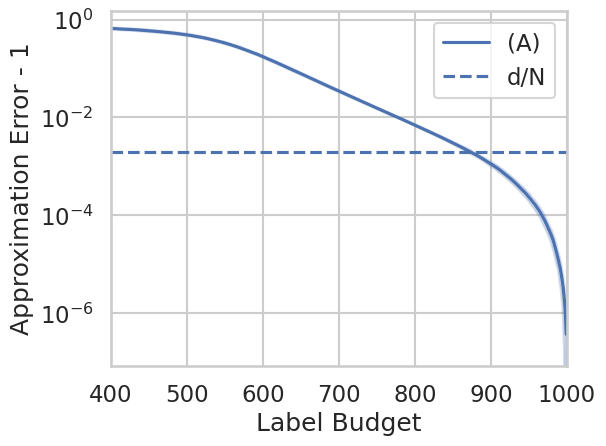
\includegraphics[width=0.4\textwidth]{figures/moons.png}}\qquad
  \subfloat[Synthetic Regression\label{fig:b}]{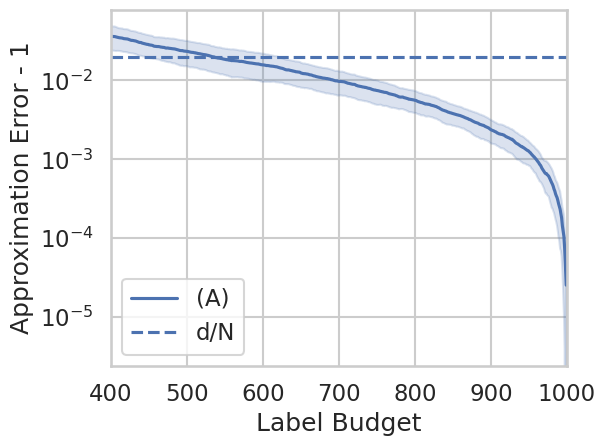
\includegraphics[width=0.4\textwidth]{figures/synthetic_regression.png}}
\caption{Synthetic datasets. In \ref{fig:a}, we only remove roughly 10\% of the rows before we reach the approximation ratio, this is likely due to being a classification problem. In \ref{fig:b}, we can remove nearly 50\% of the labels in the dataset matching our conjecture.}
\label{fig:1}
\end{figure}
\end{frame}

\begin{frame}{Real World Experiments}
\begin{figure}
  \centering
  \subfloat[Red Wine Quality\label{fig:c}]{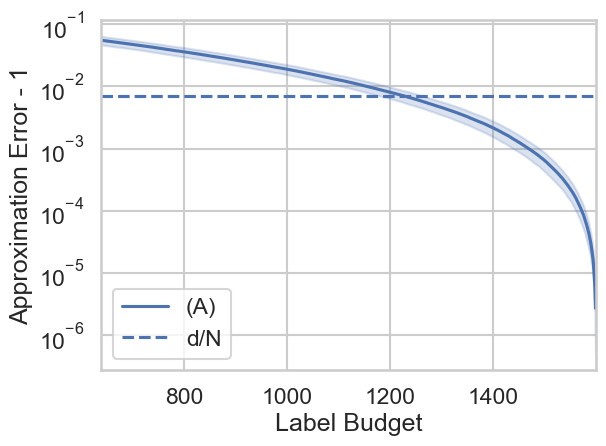
\includegraphics[width=0.3\textwidth]{figures/WineQualityRed_Fixed.png}}\qquad
  \subfloat[White Wine Quality\label{fig:d}]{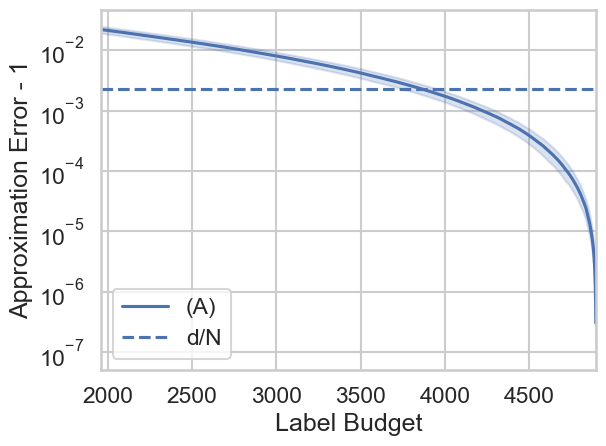
\includegraphics[width=0.3\textwidth]{figures/WineQualityWhite_Fixed.png}}\qquad
  \subfloat[Concrete Strength\label{fig:e}]{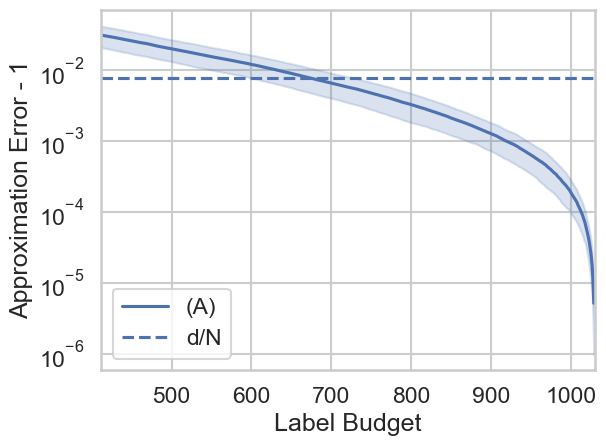
\includegraphics[width=0.3\textwidth]{figures/Concrete_Fixed.png}}
\caption{We remove roughly 30\% of the labels before our approximation ratio is achieved in the wine datasets. The concrete dataset removes roughly 50\%.}
\label{fig:2}
\end{figure}
\end{frame}

\begin{frame}{Limitations \& Future Works}
\begin{columns}
\begin{column}{0.5\textwidth}  %%<--- here
    \begin{center}
     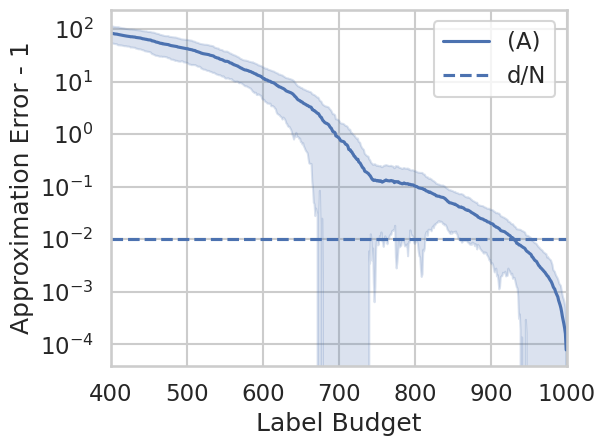
\includegraphics[width=0.9\textwidth]{figures/moons_poly.png}
     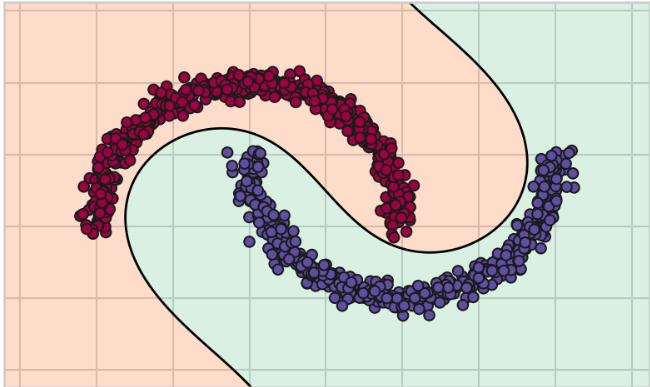
\includegraphics[width=0.7\textwidth]{figures/moons_separated.png}
          \end{center}
\end{column}
\begin{column}{0.5\textwidth}
\begin{itemize}
    \item Fitting a better regression model for the moons dataset (3rd degree polynomial) does not yield better label budget.
    \item Some synthetic datasets do not meet the necessary assumptions of this method to get a good label budget. Constants are still unknown.
    \item Developing more relaxed assumptions would be a good future work. Additional work could be done towards tightening the approximation bound's relationship to the label budget.
\end{itemize}
\end{column}
\end{columns}
\end{frame}

\section{References}
\begin{frame}[allowframebreaks]{References}
\bibliography{ref} 
\end{frame}


\begin{frame}
    \centering
    \Huge Thank You!
\end{frame}

\end{document}